%%%%%%%%%%%%%%%%%%%%%%%%%%%%%%%%%%%%%%%%%
% Masters/Doctoral Thesis
% LaTeX Template
% Version 2.5 (27/8/17)
%
% This template was downloaded from:
% http://www.LaTeXTemplates.com
%
% Version 2.x major modifications by:
% Vel (vel@latextemplates.com)
%
% This template is based on a template by:
% Steve Gunn (http://users.ecs.soton.ac.uk/srg/softwaretools/document/templates/)
% Sunil Patel (http://www.sunilpatel.co.uk/thesis-template/)
%
% Template license:
% CC BY-NC-SA 3.0 (http://creativecommons.org/licenses/by-nc-sa/3.0/)
%
%%%%%%%%%%%%%%%%%%%%%%%%%%%%%%%%%%%%%%%%%

%----------------------------------------------------------------------------------------
%	PACKAGES AND OTHER DOCUMENT CONFIGURATIONS
%----------------------------------------------------------------------------------------

% Pages (from the internal page numbering) to be printed in color - 3, 4, 5, 11, 12, 13, 14, 17, 18, 20, 21, 23, 25, 27.

\documentclass[
hidelinks,
12pt, % The default document font size, options: 10pt, 11pt, 12pt
oneside, % Two side (alternating margins) for binding by default, uncomment to switch to one side
english, % ngerman for German
doublespacing, % Single line spacing, alternatives: onehalfspacing or singlespacing
%draft, % Uncomment to enable draft mode (no pictures, no links, overfull hboxes indicated)
%nolistspacing, % If the document is onehalfspacing or doublespacing, uncomment this to set spacing in lists to single
%liststotoc, % Uncomment to add the list of figures/tables/etc to the table of contents
%toctotoc, % Uncomment to add the main table of contents to the table of contents
%parskip, % Uncomment to add space between paragraphs
%nohyperref, % Uncomment to not load the hyperref package
headsepline, % Uncomment to get a line under the header
%chapterinoneline, % Uncomment to place the chapter title next to the number on one line
%consistentlayout, % Uncomment to change the layout of the declaration, abstract and acknowledgements pages to match the default layout
]{MastersDoctoralThesis} % The class file specifying the document structure

\usepackage[utf8]{inputenc} % Required for inputting international characters
\usepackage[T1]{fontenc} % Output font encoding for international characters
\usepackage{subcaption}
\usepackage{mathpazo} % Use the Palatino font by default
\usepackage{booktabs}
\usepackage{colortbl}
\usepackage[final]{pdfpages}
\usepackage{xcolor}
\usepackage{balance}
\usepackage{epigraph}
\usepackage{alltt} % for code snippet
\usepackage{listings}
\usepackage{hyperref}
\usepackage{amsmath}
\usepackage[backend=bibtex,style=authoryear,natbib=true]{biblatex} % Use the bibtex backend with the authoryear citation style (which resembles APA)

\addbibresource{biblio.bib} % The filename of the bibliography


\usepackage[autostyle=true]{csquotes} % Required to generate language-dependent quotes in the bibliography

%----------------------------------------------------------------------------------------
%	MARGIN SETTINGS
%----------------------------------------------------------------------------------------

\geometry{
	paper=a4paper, % Change to letterpaper for US letter
	inner=4.0cm, % Inner margin
	outer=3.0cm, % Outer margin
	bindingoffset=.5cm, % Binding offset
	top=2.5cm, % Top margin
	bottom=2.5cm, % Bottom margin
	%showframe, % Uncomment to show how the type block is set on the page
}

%----------------------------------------------------------------------------------------
%	THESIS INFORMATION
%----------------------------------------------------------------------------------------

\thesistitle{Learning Support for Writing Proofs in Coq} % Your thesis title, this is used in the title and abstract, print it elsewhere with \ttitle
\supervisor{Pr. Olivier \textsc{Danvy}} % Your supervisor's name, this is used in the title page, print it elsewhere with \supname
\examiner{Dr/Pr. FirstName \textsc{LastName}} % Your examiner's name, this is not currently used anywhere in the template, print it elsewhere with \examname
\degree{B.Sc (Hons)} % Your degree name, this is used in the title page and abstract, print it elsewhere with \degreename
\author{Jeremy \textsc{Yew}} % Your name, this is used in the title page and abstract, print it elsewhere with \authorname
\addresses{} % Your address, this is not currently used anywhere in the template, print it elsewhere with \addressname

\subject{Mathematical, Computational and Statistical Sciences} % Your subject area, this is not currently used anywhere in the template, print it elsewhere with \subjectname
\keywords{Insert, keywords, here} % Keywords for your thesis, this is not currently used anywhere in the template, print it elsewhere with \keywordnames
\university{\href{https://www.yale-nus.edu.sg/}{Yale-NUS College}} % Your university's name and URL, this is used in the title page and abstract, print it elsewhere with \univname
\department{{}} % Your department's name and URL, this is used in the title page and abstract, print it elsewhere with \deptname
\group{{}} % Your research group's name and URL, this is used in the title page, print it elsewhere with \groupname
\faculty{{}} % Your faculty's name and URL, this is used in the title page and abstract, print it elsewhere with \facname

\AtBeginDocument{
\hypersetup{colorlinks=false}
\hypersetup{pdftitle=\ttitle} % Set the PDF's title to your title
\hypersetup{pdfauthor=\authorname} % Set the PDF's author to your name
\hypersetup{pdfkeywords=\keywordnames} % Set the PDF's keywords to your keywords
}

\begin{document}

\frontmatter % Use roman page numbering style (i, ii, iii, iv...) for the pre-content pages

\pagestyle{plain} % Default to the plain heading style until the thesis style is called for the body content

%----------------------------------------------------------------------------------------
%	TITLE PAGE
%----------------------------------------------------------------------------------------

\begin{titlepage}
% Fill out the titlepage.docx document, then save it as a pdf for inclusion here
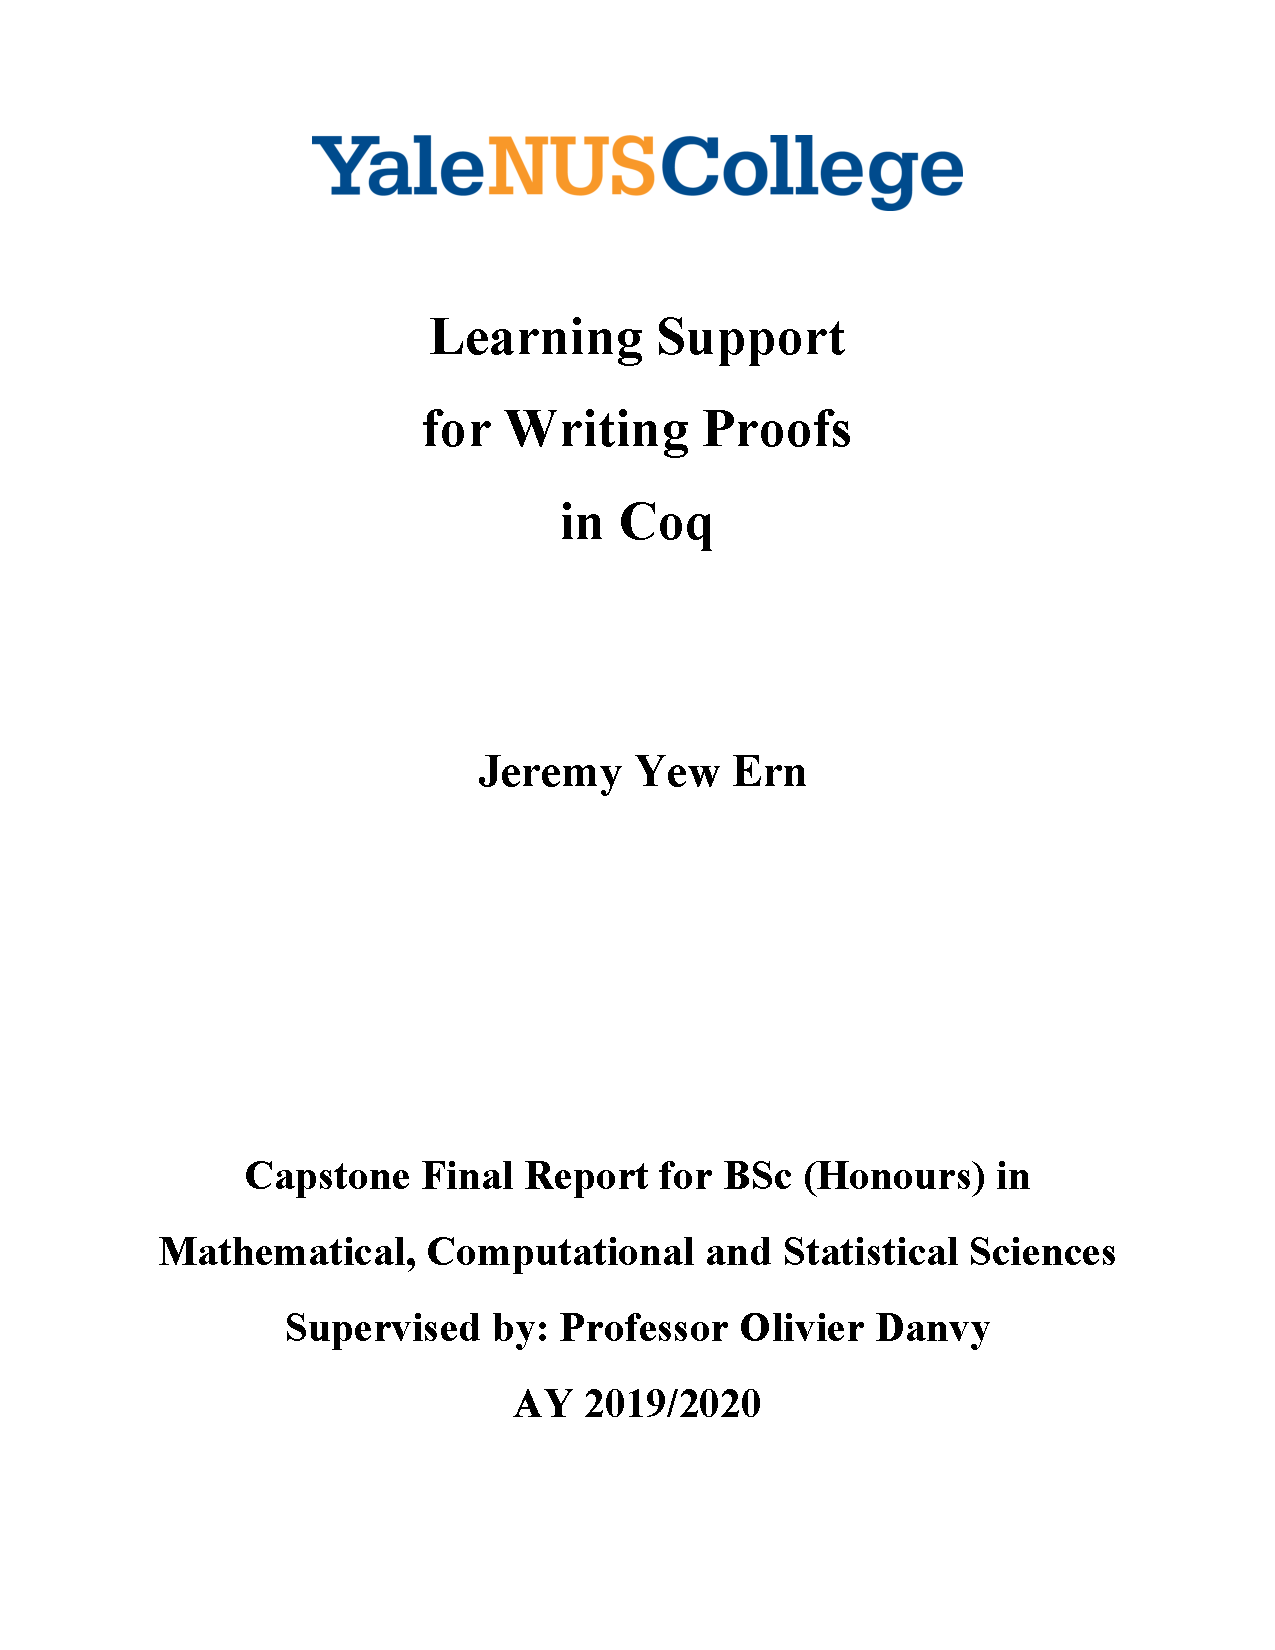
\includepdf[pages=-,pagecommand={},width=\textwidth]{titlepage.pdf}

\end{titlepage}

%----------------------------------------------------------------------------------------
%	DECLARATION & CONSENT
%----------------------------------------------------------------------------------------

% print, sign, and scan the declaration form, then include it here
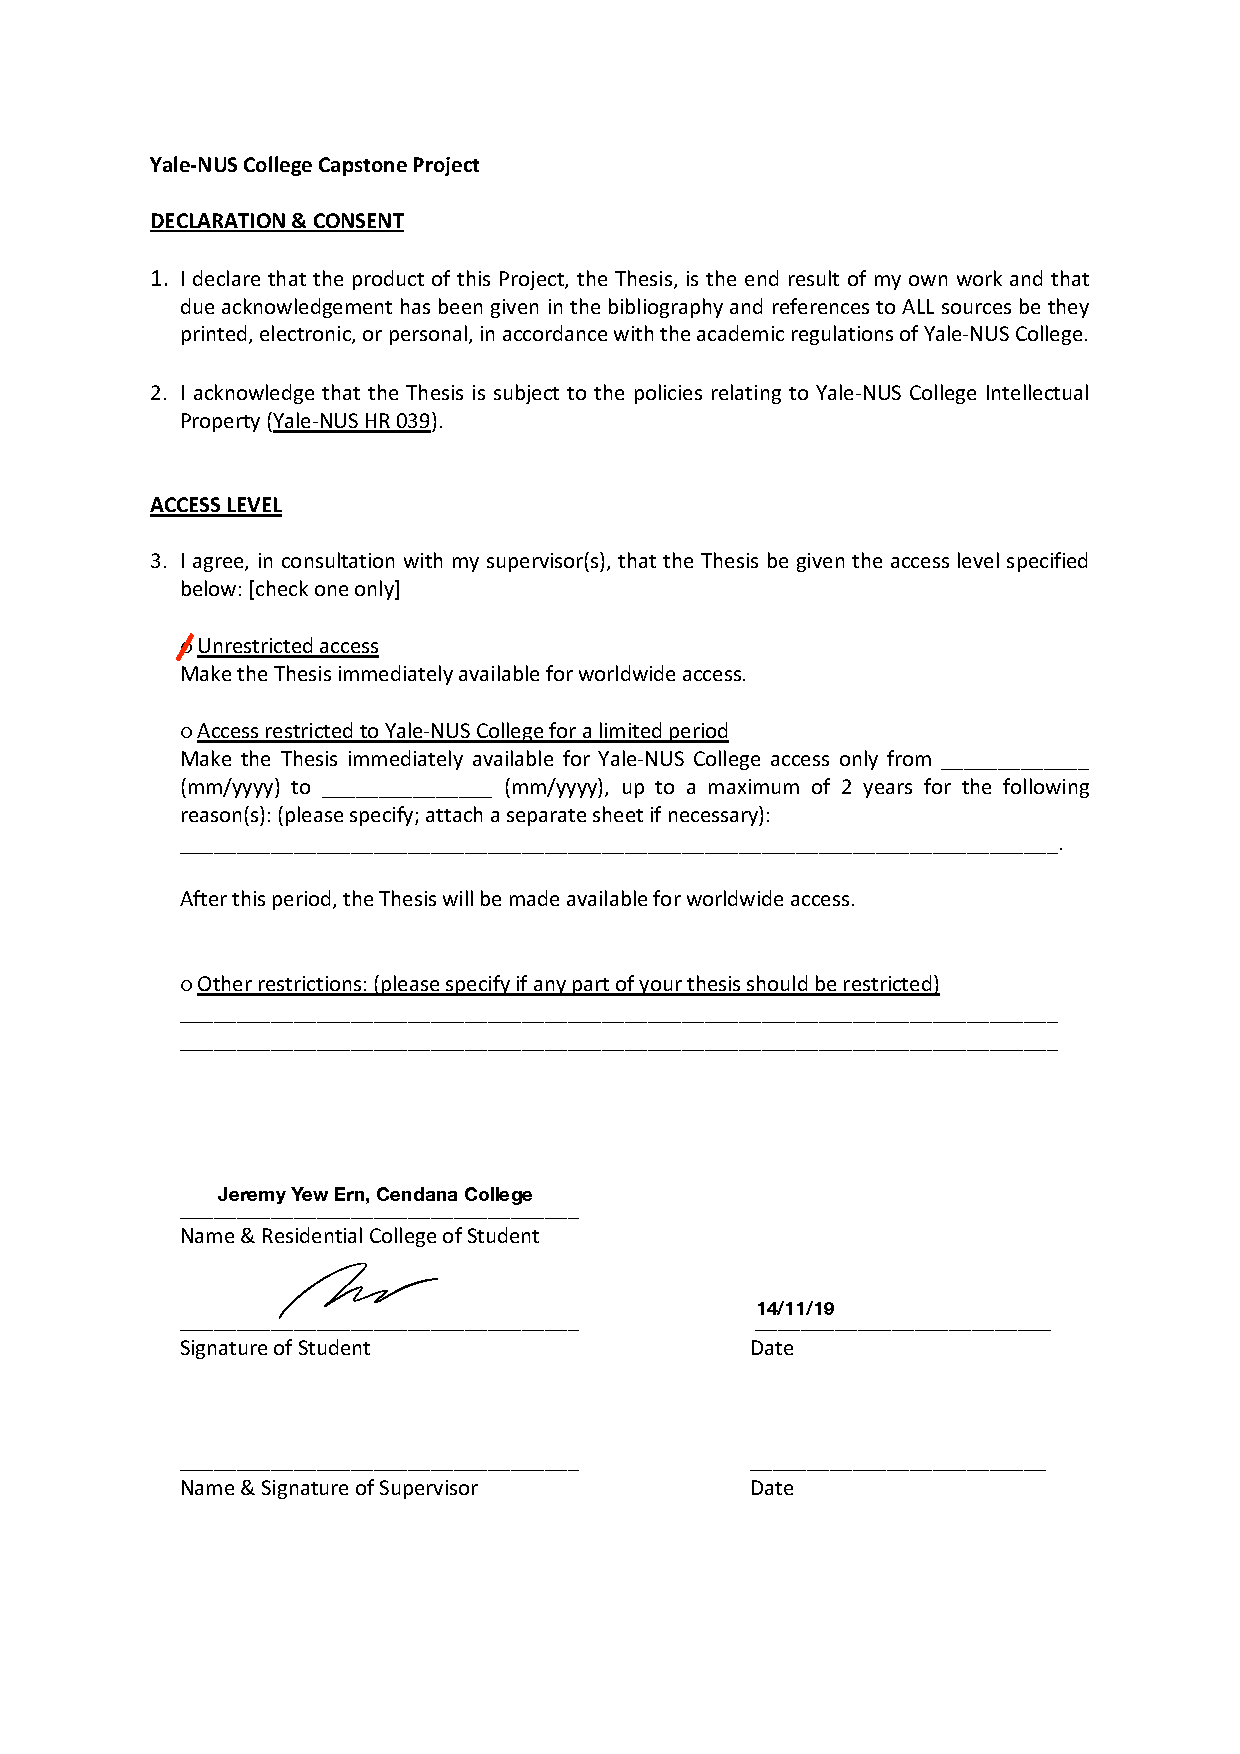
\includepdf[pages=-,pagecommand={},width=\textwidth]{declaration.pdf}

%----------------------------------------------------------------------------------------
%	ACKNOWLEDGEMENTS
%----------------------------------------------------------------------------------------

\begin{acknowledgements}
\addchaptertocentry{\acknowledgementname} % Add the acknowledgements to the table of contents
I would like to acknowledge Prof Danvy for his generous and dedicated guidance.
\end{acknowledgements}


%----------------------------------------------------------------------------------------
%	ABSTRACT PAGE
%----------------------------------------------------------------------------------------

\begin{abstract}
\addchaptertocentry{\abstractname} % Add the abstract to the table of contents
Abstract goes here.
\end{abstract}


%----------------------------------------------------------------------------------------
% CONTRIBUTIONS
%----------------------------------------------------------------------------------------

% \chapter{Claims}
%
% This paper presents the following original contributions:
%
% \begin{enumerate}
% 	\item A hardware device for haptic sensory substitution along with designs for the construction of such a system.
% 	\item Two implementations of sensory substitution using haptic feedback, continuous and delayed feedback-based spatial navigation tasks, each of which include:
% 		\begin{enumerate}
% 			\item a front-end for providing visual input to the user during the training phase with useful readouts to the researcher,
% 			\item a transmission protocol, which maps information from the task at hand (spatial coordinates, velocity information, etc) to time-based sensor actuation signals (20$^{\circ}$ on servo 1, 35$^{\circ}$ on servo 2, etc) in real-time.
% 		\end{enumerate}
% 	\item An evaluation framework for measuring the performance of a sensory substitution system, which provides sample tasks that can be used to standardise and compare performance across the board for future research.
% 	\item A review of existing hardware and software stacks as well as possible avenues for development based on the developed metrics.
% \end{enumerate}
%
% In addition, code for displaying results in real-time, modules for managing servo overload, network latency and other factors were also written by the author.


% %----------------------------------------------------------------------------------------
% %	DECLARATION PAGE
% %----------------------------------------------------------------------------------------
%
% \begin{declaration}
% \addchaptertocentry{\authorshipname} % Add the declaration to the table of contents
%
% \noindent I, \authorname, hereby declare that this Project, the Capstone Report and associated work listed herein, is the end result of my own work and that due acknowledgement has been given in the bibliography and references to ALL sources printed, electronic, or personal, in accordance with the academic regulations of Yale‐NUS College.
% I acknowledge that the Thesis is subject to the policies relating to Yale‐NUS College Intellectual  Property (Yale‐NUS HR 039).
%
%
% % I confirm that:
% %
% % \begin{itemize}
% % \item This work was done wholly or mainly while in candidature for a research degree at this University.
% % \item Where any part of this thesis has previously been submitted for a degree or any other qualification at this University or any other institution, this has been clearly stated.
% % \item Where I have consulted the published work of others, this is always clearly attributed.
% % \item Where I have quoted from the work of others, the source is always given. With the exception of such quotations, this thesis is entirely my own work.
% % \item I have acknowledged all main sources of help.
% % \item Where the thesis is based on work done by myself jointly with others, I have made clear exactly what was done by others and what I have contributed myself.\\
% % \end{itemize}
%
% \noindent Signed:\\
% \rule[0.5em]{25em}{0.5pt} % This prints a line for the signature
%
% \noindent Date:\\
% \rule[0.5em]{25em}{0.5pt} % This prints a line to write the date
% \end{declaration}
%
% \cleardoublepage

%----------------------------------------------------------------------------------------
%	QUOTATION PAGE
%----------------------------------------------------------------------------------------

% \vspace*{0.2\textheight}
%
% \noindent\enquote{\itshape Thanks to my solid academic training, today I can write hundreds of words on virtually any topic without possessing a shred of information, which is how I got a good job in journalism.}\bigbreak
%
% \hfill Dave Barry

%----------------------------------------------------------------------------------------
%	LIST OF CONTENTS/FIGURES/TABLES PAGES
%----------------------------------------------------------------------------------------

\tableofcontents % Prints the main table of contents

% \listoftables % Prints the list of tables
\label{lst:tabs}

% \listoffigures % Prints the list of figures
\label{lst:figs}

%----------------------------------------------------------------------------------------
%	ABBREVIATIONS
%----------------------------------------------------------------------------------------

% \begin{abbreviations}{ll} % Include a list of abbreviations (a table of two columns)
%
% \textbf{LAH} & \textbf{L}ist \textbf{A}bbreviations \textbf{H}ere\\
% \textbf{WSF} & \textbf{W}hat (it) \textbf{S}tands \textbf{F}or\\
%
% \end{abbreviations}

%----------------------------------------------------------------------------------------
%	PHYSICAL CONSTANTS/OTHER DEFINITIONS
%----------------------------------------------------------------------------------------

% \begin{constants}{lr@{${}={}$}l} % The list of physical constants is a three column table
%
% % The \SI{}{} command is provided by the siunitx package, see its documentation for instructions on how to use it
%
% Speed of Light & $c_{0}$ & \SI{2.99792458e8}{\meter\per\second} (exact)\\
% %Constant Name & $Symbol$ & $Constant Value$ with units\\
%
% \end{constants}

%----------------------------------------------------------------------------------------
%	SYMBOLS
%----------------------------------------------------------------------------------------

% \begin{symbols}{lll} % Include a list of Symbols (a three column table)
%
% $a$ & distance & \si{\meter} \\
% $P$ & power & \si{\watt} (\si{\joule\per\second}) \\
% %Symbol & Name & Unit \\
%
% \addlinespace % Gap to separate the Roman symbols from the Greek
%
% $\omega$ & angular frequency & \si{\radian} \\
%
% \end{symbols}

%----------------------------------------------------------------------------------------
%	DEDICATION
%----------------------------------------------------------------------------------------

% \dedicatory{Dedicated to ceux l\`{a} qui veulent.}

%----------------------------------------------------------------------------------------
%	THESIS CONTENT - CHAPTERS
%----------------------------------------------------------------------------------------

\mainmatter % Begin numeric (1,2,3...) page numbering

\pagestyle{thesis} % Return the page headers back to the "thesis" style

% Include the chapters of the thesis as separate files from the Chapters folder
% Uncomment the lines as you write the chapters

% Chapter Template

\chapter{Introduction} % Main chapter title

\label{intro} % Change X to a consecutive number; for referencing this chapter elsewhere, use \ref{ChapterX}

%----------------------------------------------------------------------------------------
%	SECTION 1
%----------------------------------------------------------------------------------------

\section{Introduction}
The goal of this research project is to provide learning support for students enrolled in YSC3216: Functional Programming and Proving (FPP), by building a tool that checks for syntax issues in student's proof submissions.

FPP is a course in Yale-NUS College taught by Professor Olivier Danvy, under the Mathematical, Computational and Statistical Sciences major. FPP introduces students to the Coq proof assistant, which is a system for writing and verifying formal proofs. 

The learning goal for the first half of the course is to build muscle memory for basic proof techniques and programming habits. 

To this end, I implement a program that can act as a set of 'safety rails' to guide students towards developing the proper muscle memory. In particular, the program will enforce explicit tactic application within a subset of Coq, amongst other syntax rules. The Lecturer will be able to provide a grammar specification as an input to the tool. The program will be written as an extension of the Emacs text editor, and can therefore be used by students interactively. 
%-----------------------------------
%	SUBSECTION 1
%-----------------------------------
\section{Context}
\subsection{Functional programming (FP)}
Functional programming is a programming paradigm that models programs as mathematical functions. That is, a program defines a mapping of every possible input to exactly one output value. Functional programming is partly characterized by its 'declarative' style, in which the programmer directly expresses the desired output, derived from the input.

Students taking FPP are expected to have completed Intro to Computer Science taught in Yale-NUS, which trains them in functional programming with the language OCaml. Coq has a language of programs that is very similar to OCaml, and is in fact written in OCaml. 

\subsection{Proving}
In mathematics, a proposition is a statement that either holds or does not hold; a proposition is also sometimes called a theorem or lemma. 

Proofs can be defined as a logical argument about whether a proposition holds. Proofs use logical rules to demonstrate that what we are sure of (an axiom) implies the truth of something we were not sure of. 

In mathematical proofs, propositions often contain equations, which are statements asserting the equality of two expressions containing variables (unknown values). In equational reasoning, we apply axioms to equations in order to incrementally transform them into something that is clearly true. 

\subsection{Verifiable proofs with the Coq proof assistant}
Many proofs in mathematics or computer science are natural language proofs - that is, they are written in a natural language, like English. Even though they may use jargon and formal symbols, they may be considered informal. Since natural languages are often ambiguous, natural language proofs are susceptible to misinterpretation or misconception. Furthermore, informal proofs rely on humans to check for logical errors, but humans are fallible.

On the other hand, just as there programming languages that express a set of instructions to be executed by a computer, there are also domain-specific languages for writing formal proofs that can be automatically, or mechanically, verified by a computer. 

Therefore Coq allows us to write formal, verifiable proofs in a structured logical language called Gallina, and will also automatically verify that our proofs are correct. 

Proving is done as such: 
1. First, we state a theorem (or lemma, proposition, etc) in the logical language of Coq. 
2. Then, we solve 'subgoals'  generated by Coq (sub-statements we need to prove in order to prove the theorem) by stating a sequence of 'tactics' (the method we use at each step). As we apply each tactic to the current subgoal (by executing each line of code), Coq will progressively transform the subgoal.
3. Once all our subgoals have been transformed into something that is clearly true, our proof is complete. Every proof step has been demonstrated to progress logically from each other; this process can be reproduced by any other user executing the same proof. Thus the the proof is verifiably correct. 


\subsection{YSC3236 Functional Programming and Proving (FPP)}
FPP is a course in Yale-NUS College taught by Professor Olivier Danvy, under the Mathematical, Computational and Statistical Sciences major. The class is taken not only by Yale-NUS students, but also PhD and post-doctoral students from the National University of Singapore (NUS) School of Computing (SoC). 

FPP introduces students to the Coq proof assistant. Through the course, students gain an appreciation for the interconnectedness of computer programs and logical proofs - which have previously been presented to them as distinct domains of knowledge. For example, they are led to realize that an explicitly written Coq proof exactly corresponds to an equivalent mathematical proof they have written in detail, by hand.
  
Students engage in weekly assignments consisting of rigorous, progressive exercises involving:
\begin{itemize}    
    \item writing mathematical proofs
    \item  writing programs, and proofs about the properties of programs
    \item eventually, stating their own theorems and proving them
\end{itemize}

\subsection{GNU Emacs Editor}   

Emacs is a family of real-time text editors which are characterized by their customizability and extensibility. GNU Emacs was written in 1984 by GNU Project founder Richard Stallman. 

The user interacts with files displayed in 'buffers' - a view of a text file - via **commands** invoked by 'macros' - keystroke sequences. Feedback and status messages are displayed in a smaller buffer at the bottom of the screen - the 'minibuffer'. The user can create and dismiss buffers, and multiple buffers can exist without all being on display.  

\begin{itemize}
    \item Emacs is customizable because users can change the behaviour of some commands via parameters, without having to redefine or modify the underlying code of the command itself. Users can also easily redefine key mappings.
    \item Emacs is extensible because users can write new commands as programs and bind them to new macros. 
    \item GNU Emacs provides a language based on Lisp, Emacs Lisp, that is used to write extensions/programs run within Emacs. 
\end{itemize}

GNU Emacs is used in Intro CS, Intro to Algos and Data Structures, and FPP, so students are expected to have familiarity with its interface and indeed will be required to use it, since the class uses the Proof General interface. 


\subsection{Proof General}   
Proof General is a powerful, configurable and generic Emacs interface for proof assistants, developed at the University of Edinburgh since 1992. It provides a common interface across various proof assistants, including Coq, and allows users to interactively edit proof scripts. 

The interface presents users with three buffers (windows): one buffer in which the Coq script is to edited, one buffer to display subgoals, and one buffer to display other responses like search results or error messages.
% Chapter Template

\chapter{Building muscle memory} % Main chapter title

\label{building-muscle-memory} % Change X to a consecutive number; for referencing this chapter elsewhere, use \ref{ChapterX}

%----------------------------------------------------------------------------------------
%	SECTION 1
%----------------------------------------------------------------------------------------

\section{A skilled discipline}
The learning philosophy of FPP is that programming and proving is similar to training in any skilled discipline such as martial arts, cooking, or dance: beginner training should build muscle memory for basic skills and habits. 

For example, if you are training to be a chef, but you don't develop proper knife skills early on, this will hurt you for the rest of your career. 

Therefore, in the first half of the course, students complete rigorous, progressive exercises in order to practice specific proof techniques and programming habits. In the second half of the course, students can then rely on this muscle memory to write proofs with greater creativity and efficiency. By the end of the course, students will have independently written more proofs than they have ever written in their lives, and all of these proofs would have been verified by Coq.

% Chapter Template

\chapter{Writing proofs} % Main chapter title

\label{writing-proofs} % Change X to a consecutive number; for referencing this chapter elsewhere, use \ref{ChapterX}

%----------------------------------------------------------------------------------------
%	SECTION 1
%----------------------------------------------------------------------------------------

\section{What could go wrong?}
With programming languages, there are usually many ways to write the same program. In the same way, there are many equivalent representations of a Coq proof, because Coq is flexible and allows you to take shortcuts. However, for new learners, this flexibility can be counterproductive. In the context of FPP, several issues arise. 

\subsection{Abuse of tactics}
First, students may abuse tactics that have not been introduced in the course. 

When students get stuck on a proof, they might Google for related solutions or search the Coq documentation for anything that will 'solve' the proof. They might end up using a magical tactic, for example `trivial`, as in the latter version of the example proof below. 
\begin{verbatim}
Lemma SSSn_is_3_plus_n :
  forall n : nat,
  S (S (S n)) = 3 + n.
Proof.
  intro n.
  rewrite <- (Nat.add_1_l n).
  rewrite <- (plus_Sn_m 1 n).
  rewrite <- (plus_Sn_m 2 n).
  reflexivity.
Qed.
\end{verbatim}

\begin{verbatim}
Lemma SSSn_is_3_plus_n :
  forall n : nat,
  S (S (S n)) = 3 + n.
Proof.
  trivial.
Qed.
\end{verbatim}

Under the hood, the `trivial` tactic uses some heuristics to automatically try various strategies to solve the current formula. However, in the first half of the course the focus is for students to understand every single proof step they write, because if students cannot explain what they are doing, they do not really understand it. Therefore, using a tactic like `trivial` completely goes against the objective of the exercise. 

Yet these tactics still appear in student submissions, because they might still have the bad programmer mindset of "if it works, its fine". This causes time between resubmissions to be wasted on superficial feedback. 

\subsection{ Misuse of tactics }
Second, even when students use tactics that have been introduced, they may misuse them by taking shortcuts.

For instance, the rewrite tactic is used to apply a rule to the current formula. A rewrite rule is a function that expects specific terms in the formula as arguments; Coq will rewrite the given terms. For example, the rewrite rule below accepts three arguments, n, m, p.

\begin{verbatim}
Check Nat.add_assoc.
# Nat.add_assoc : forall n m p : nat, n + (m + p) = n + m + p. 
\end{verbatim}

However, Coq is flexible with the number of arguments you give it. As the example proofs below demonstrate, you could give the rewrite rule three, two, one or zero of the rewrite arguments required, and Coq will simply pick the first terms in the formula that it can apply the rule to. 
\begin{verbatim}
Proposition add_assoc_nested :
  forall a b c d e: nat,
    a + b + c + d + e = 
    a + (b + (c + (d + e))).
Proof.
  intros a b c d e.
  rewrite -> (Nat.add_assoc a b (c + (d + e)) ).
  rewrite -> (Nat.add_assoc (a + b) c (d + e) ).
  rewrite -> (Nat.add_assoc (a + b + c) d e ).
  reflexivity.
Qed.
\end{verbatim}
\begin{verbatim}
Proposition add_assoc_nested :
  forall a b c d e: nat,
    a + b + c + d + e = 
    a + (b + (c + (d + e))).
Proof.
  intros a b c d e.
  rewrite -> (Nat.add_assoc a b )
  rewrite -> (Nat.add_assoc (a + b) ).
  rewrite -> Nat.add_assoc.
  reflexivity.
Qed.
\end{verbatim}
However, in the first half of the course, the focus is on understanding the proof at a low level. Clearly, students need to be aware of exactly which terms they have changed at every step. Otherwise, they may get stuck in a proof because they applied a rewrite rule to the wrong term, or they might reach a solution without knowing how. Therefore, taking advantage of this shortcut goes against the spirit of the exercise. 

Furthermore, this issue is not easy to check manually, especially with assignments that are hundreds of lines long.

These two issues - abuse and misuse of tactics - correspond to issues of **abstract syntax** (what language constructs are represented in the grammar) and **concrete syntax** (what structures are used to represent language constructs) respectively. 

Therefore, it would be nice to have a system that can anticipate and identify both abstract and concrete syntax issues, to save both students and the Lecturer's time and help achieve the learning goals of the course.   


\subsection{Other issues}
Other issues I have discussed with the Lecturer include: 
\begin{itemize}
  \item arbitrary indentation levels for proof subcases 
  \item inconsistent naming
  \item breaking style conventions. 
\end{itemize}


All these issues seem to persist across the progression of the module, as well as iterations of the module, despite the Lecturer explaining to the students the rationale for following provided syntactical guidelines, and repeated reminders.

The idea is for the proposed tool to cut down on the amount of **'superficial'** feedback - e.g., 'don't use this tactic, because...', or 'this is bad style, please correct it in this way', etc. - that the Lecturer must give repeatedly to individual students, and instead automatically lead students towards solutions that only require **substantive** feedback - e.g., ideas to pursue, possible restructuring of the proof, etc. The less superficial feedback is required, the more time the Professor can spend on providing substantive feedback. Also, students will spend less effort correcting style errors if they do so immediately.

Yet, superficial feedback is not merely incidental. Superficial feedback reflects the formal concerns of the course and helps reinforces good programming habits, which will not only assist the learning experience of students, but benefit them in future endeavors. Therefore, the tool does not simply emphasize pedantic concerns; it makes concrete the formal training prescriptions of the course. 
% Chapter Template

\chapter{Solution} % Main chapter title

\label{solution} % Change X to a consecutive number; for referencing this chapter elsewhere, use \ref{ChapterX}

%----------------------------------------------------------------------------------------
%	SECTION 1
%----------------------------------------------------------------------------------------


\section{A grammar of grammars}
The solution to these issues of abstract and concrete syntax is to develop a system that enforces explicit tactic application within a subset of Coq, amongst other rules. This system will be in the form of a program that takes as input a student's Coq file, as well as a grammar specification provided by the Lecturer. It will output warnings about instances where a syntax rule has been violated. (From here, I refer to 'the program' interchangeably as 'the tool' or 'the parser'.)

The program will be writen as an extension of the Emacs editor, so students can execute a command within Emacs to parse the current file, and thus use the tool interactively as they construct their proofs. 

The program will thus act as a set of safety rails for students to develop the right habits, in the spirit of learning for the first half of the course. As a result, students will have earlier, automated intervention on syntactical issues in their assignments, and the Lecturer can spend more time on substantive rather than superficial feedback. 

However, the parser should not 'hard-code' a grammar that only enforces particular syntax rules. Instead, it should accept and parse a grammar specification that is readable and easily editable, and enforce that grammar. In other words, we need to implement a grammar of grammars. This will allow the Lecturer to modify existing rules or extend them, without having to modify the source code of the parser. This will also make it easier for other course instructors or developers to modify the parser behaviour for their own needs. 

\section{Implementation trade-offs}
The first trade-off is whether to write a custom syntax parser by hand, or to use a parser generator.

A parser generator is a program that accepts a grammar specification as input, and automatically generates a parser that implements the grammar. I have identified parser generators intended to be run within Emacs, and written in Emacs Lisp (more on that below).

A parser generator would be ideal - we do not want to reinvent the wheel. Firstly, in theory, there is minimal to no programming to be done. Instead, we declare a grammar using some notation. 

Secondly, relying only on the declared grammar makes the program more extensible; it is easier for the Lecturer or other developers to modify existing rules or add new rules, since they do not need to touch underlying code.

However, it will be necessary to grasp the grammar that is required as input in the first place. 

A second trade-off relates to the case where we write a custom parser by hand: whether to write it using Emacs Lisp, or another language that I am more familiar with.

Of course, using a familiar language might mean that we get to a first working version faster. But an Emacs Lisp implementation has many benefits: 
\begin{itemize}
    \item Easier for other Emacs developers to build on  
    \item Integrated with Emacs editor features
    \item Run within Emacs. No need to call external process, no external dependencies, no interoperability issues (e.g. making a call to create a new thread, etc).  
\end{itemize}


This is why it is ideal to use a parser generator that generates Emacs Lisp code.  

\section{Current progress}
I have made progress in the following areas: 

\begin{itemize}
    \item Defining a subset of Coq grammar.
    \item Exploring different types of parsers for different types of languages.
    \item How to write a parser.
    \item How to write Emacs Lisp programs.
    \item How to write an Emacs extension.
\end{itemize}


In particular, I have written a script in Emacs Lisp that registers an Emacs interactive command, which may be executed while editing a Coq proof. The command is able to take the current buffer and use the Coq shell to parse it for Coq syntax errors. This command would be eventually used to run our custom parser; the idea is to first check that the input is syntactically correct with respect to Coq's grammar. This allows us to develop our custom parser assuming that the input code is already syntactically correct, hence we may define or provide a grammar that only encompasses a subset of Coq's grammar.

Additionally, I have also started trying to use the Semantic Bovine parser generator. Semantic is a framework for writing Emacs packages, and Bovine is a built-in parser generator provided by Semantic. It accepts a BNF (Backus-Naur Formation)-like grammar specification, and generates a parser in Emacs Lisp, which is ideal. The main obstacle for now would be the slightly obscure documentation. The first step I am aiming for would be to specify a simple grammar (such as for arithmetic expressions with infix notation), and ensure that it raises an appropriate error when given a syntactically incorrect input. 

\section{Challenges ahead}
The challenges ahead would be to decide on and proceed with an implementation of a program that can enforce a grammar addressing the two issues mentioned. Following which, I can then explore other rules mentioned. I will also be iterating on the tool based on usability feedback from both the Lecturer and FPP students, and the feedback will also be the measure of success for my project.
% % Chapter 1

\chapter{Tips} % Main chapter title
\epigraph{``Y a plein de c\^otes \`a Ibiza\\C'est vraiment dur il fait tr\`es chaud.''}{\textit{Zambla}}

\label{chapter1} % For referencing the chapter elsewhere, use \ref{Chapter1}

%----------------------------------------------------------------------------------------
\section{Introduction}
hi hi
Dear student reading that chapter, greetings!
After doing some research and writing reports for more than 12 years, I realized that LaTeX is the second worst way to write a thesis.
The worst one is Word.
Then you may be wondering, which is the best way to write a report?
Well, actually there is no best way.
Hence you are stuck with LaTeX.

\subsection{Goal of this chaper}
In this chapter, I will demonstrate a few interesting features of LaTeX, and more importantly, provide examples of Figures, Tables, Equations and Code Snippets.
These may be easy to deal with on Word, but here it is another story.
The general idea is to keep these examples, copy-paste them, then modify them to fit your needs.
If you are seeing this content while reading \texttt{main.pdf}, please load the overall LaTeX project in your LaTeX editor, and open the \texttt{chapters/chaper1.tex}.
\\
\\
Done?
Ok let us move on then!
So by now, you should have noticed a few things:
\begin{itemize}
  \item Each sentence of the text is on a distinct line. Yet, sentences are still within the same paragraph.
  \item Backslash is an escape character, used at the beginning of LaTeX commands.
  \item To end a paragraph (or actually insert a newline), we can use the \textbackslash{}\textbackslash{} command.
\end{itemize}
Also now you know how to do a bullet list.

\subsection{Structure of a chapter}
Chapter contain sections (defined with \textbackslash{}section\{Name of your section\}), subsections (\textbackslash{}subsection).

\subsubsection{Because subsubsection that's why!}
Subsubsections are also available (\textbackslash{}subsubsection).

\paragraph{Paragraph}
If you really insist, there are also paragraphes, which may or may not be the same as a subsubsection.
Note that the automatically generated table of contents only goes to two levels of depth within chapters by default.
This can be changed, but you likely do not want to do that.

\subparagraph{Subparagraph}
I was today years old when I discovered the subparagraph. Seriously, do not use it.

\section{Font Formatting Commands}
Similarly to Word, LaTeX provides simple formatting, including \textbf{bold}, \textit{italic}, \underline{underlined} and \texttt{ugly stuff}.
However, no underline or strikethrough by default.
You can also change the size of the text, using {\tiny tiny}, {\small small}, {\large large}, {\huge huge}.
These last commands work within a specific scope.
The scope can be specified using \{ and \}, with the \{ placed before the \textbackslash{}size command.

\subsection{Special characters}
LaTeX uses 10 special characters. Each of these characters has a special meaning.
\begin{enumerate}
  \item Ampersand (\&) is used in tables as a cell delimiter.
  \item Percent sign (\%) is used for commenting a line.
  \item Dollar sign (\$) is used to switch back/from mathematical notation mode.
  \item Hash sign (\#) is used to create macros --- you definitely do not want to go more in depth here.
  \item Underscore (\_ or \textunderscore) is used to indicate a subscript in maths mode, if you use it in text mode ( without using backslash in front to ''escape'' it), your project will not compile anymore. \textbf{You may want to read that twice, and remember it.} It is in a LaTeX template, therefore it must be true.
  \item Curly brackets (\{ and \}) or bracets are used by LaTeX commands, as you likely already noticed.
  \item Tilde (\textasciitilde) can be used to create a non-breaking space (so that both words are on the same line).
  \item Caret/Circumflex/Hat (\textasciicircum) is used to indicate superscript (exponent) in maths mode.
  \item Backslash (\textbackslash) is used in front of every command. You cannot simply escape it to print it, as \textbackslash{}\textbackslash{} create a new line.
\end{enumerate}
If you happen to insert some of these symbols in your text without either escaping (when possible) or using the correct command, your project will likely not compile.
Thus, you may want to be extra careful about that problem.
Note: the underscore issue may also be encountered with bibliography.
So if \texttt{bibtex} displays an error, it may also come from an underscore somewhere in the abstract, DOI or URL field.

\section{Equations}
Here is an equation:
\begin{equation}
\int_0^\infty e^{-x^2} dx
\label{eq:eq1}
\end{equation}

I could also want to have this equation inline, i.e. within the text: $\int_0^\infty e^{-x^2} dx$.
In that case, simply use \textdollar{} (by the way, note that using the dollar sign in your text switches to mathematical notation. To actually print a dollar sign use the \textbackslash{}textdollar command).
The equation above has a label, meaning you can refer to it. The numbering system uses the chapter number (in this case 1), then the equation position within the chapter (1 again).
Example: Equation~\ref{eq:eq1} is an example of an equation in LaTeX{}.
In case you would like to have an equation without numbering it? Easy!
\begin{equation*}
t = a \times log_{2}(\frac{D}{W} + 1) + b
\end{equation*}

The only difference? The \textasteriskcentered{}  symbol in the \textbackslash{}begin\{equation\textbf{\textasteriskcentered}\}.
This also works with Figures and Tables.

\section{Code Snippets}

\begin{lstlisting}
  int main (int argc, char ** argc)
  {
    printf("Hello world!\n");
    return 0;
  }
\end{lstlisting}

This template uses the \texttt{lstlisting} package, which not the best for code snippets.
However, it works without any problem, while other packages may have compatibility issues.
Feel free to try alternative solutions, the best one being \texttt{minted}.

\section{Figures}
Figures are a bit tricky with LaTeX {\tiny(not as much as tables though)}.
Let us see a simple example below:
\begin{figure}[!h]
  \centering
    
\includegraphics[width=0.9\textwidth]{figures/future.png}
  \caption{When a YNC alumni tells you that back in their days, they did not have LaTeX template and would write their report in latin on a papyrus.}
  \label{fig:future}
\end{figure}
You can refer to it: Figure~\ref{fig:future}.
This is possible thanks to the \textbackslash{}label command.
The figure should also be shown on the \hyperref[lst:figs]{List of Figures} page (note this other way of referring to another part of the manuscript!).
A common practice is use the following naming convention:
\begin{itemize}
  \item A prefix, indicating the nature of the object labelled: \texttt{eq} for equations, \texttt{fig} for figures, \texttt{tab} for tables.
  \item A colon.
  \item A unique name (easy to remember) describing your figure. Example: exp1confmatrix would suggest that the figure shows a confusion matrix for your experiment 1.
\end{itemize}

A few other points: The \textbackslash{}caption and \textbackslash{}label can be put either before or after the \textbackslash{}includegraphics command.
When you create a Figure, you need to provide placement information for LaTeX. LaTeX will usually not locate the figures \emph{exactly} where you want them.
The most common specifiers are: \texttt{h} (here), \texttt{b} (bottom of the page) and \texttt{t} (top). The \texttt{!} specifier tries to force LaTeX to put the image exactly at the location you specified (with mixed success though).
For a longer list of specifiers, please refer to: \url{https://en.wikibooks.org/wiki/LaTeX/Floats,_Figures_and_Captions}.

\subsection{Figure Size}
The size of the figure can be determined by the first parameter of the \textbackslash{}includegraphics command.
In this example, we set the size to be $0.9 \times \texttt{textwidth}$, or 90\% of the size of a column.
We could have used an absolute value in cm, e.g. \texttt{width=19cm}.

\subsection{Supported Formats}
Use standard formats, such as PNG, PDF, JPG.
LaTeX also supports other formats, such as EPS.
\textbf{Rule of thumb: use PDF as much as you can, as it uses vector graphics, making it easy to scale the figure to very large format without problems.}

\subsection{Multiple images in one figure}
You can also create complex figures with multiple images.
Here is an example, which uses a $2\times2$ layout.
The overall figure can be referred as Figure~\ref{fig:drake}.
\begin{figure}[!h]
  \begin{subfigure}[t]{.5\textwidth}
    \centering
    
\includegraphics[width=\linewidth]{figures/draketl.png}
    %\caption{We could totally insert a caption here}
    %\label{fig:draketl}
  \end{subfigure}
  \hfill
  \begin{subfigure}[t]{.5\textwidth}
    \centering
    
\includegraphics[width=\linewidth]{figures/draketr.png}
    %\caption{We could totally insert a caption here}
        %\label{fig:draketr}
  \end{subfigure}

  %\medskip
  % the medskip will have white space between both lines
  \begin{subfigure}[t]{.5\textwidth}
    \centering
    
\includegraphics[width=\linewidth]{figures/drakebl}
    %\caption{We could totally insert a caption here}
        %\label{fig:drakebl}
  \end{subfigure}
  \hfill
  \begin{subfigure}[t]{.5\textwidth}
    \centering
    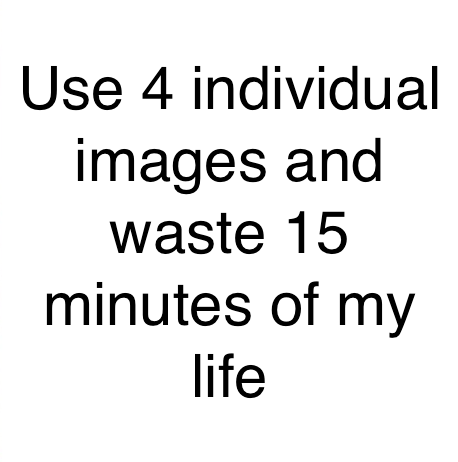
\includegraphics[width=\linewidth]{figures/drakebr}
    %\caption{We could totally insert a caption here}
    %\label{fig:drakebr}
  \end{subfigure}
  \caption{Example of a complex figures on a $2\times2$ layout.}
  \label{fig:drake}
\end{figure}

\section{Tables}
Tables can be a nightmare in LaTeX.
The easiest way to deal with tables in LaTeX is to use some online tools.
My favorite so far: \url{https://www.tablesgenerator.com/}

Here is an example of confusion matrix generated:
\begin{table}[!h]
  \resizebox{\textwidth}{!}{
\begin{tabular}{|c|c|ccccccccc}
\cline{1-2}
Chest (C)                         & -     &                                                                          &                                                                           &                                                                          &                          &                            &                           &                           &                            &                                                                            \\ \cline{1-3}
Chest (ND)  & *     & \multicolumn{1}{c|}{-}                                                   &                                                                           &                                                                          &                          &                            &                           &                           &                            &                                                                            \\ \cline{1-4}
Chest (D)   & *     & \multicolumn{1}{c|}{-}                                                   & \multicolumn{1}{c|}{*}                                                    &                                                                          &                          &                            &                           &                           &                            &                                                                            \\ \cline{1-5}
Ear          & -     & \multicolumn{1}{c|}{-}                                                   & \multicolumn{1}{c|}{-}                                                    & \multicolumn{1}{c|}{}                                                    &                          &                            &                           &                           &                            &                                                                            \\ \cline{1-6}
Thigh       & *     & \multicolumn{1}{c|}{-}                                                   & \multicolumn{1}{c|}{*}                                                    & \multicolumn{1}{c|}{*}                                                   & \multicolumn{1}{c|}{-}   &                            &                           &                           &                            &                                                                            \\ \cline{1-7}
Neck        & -     & \multicolumn{1}{c|}{*}                                                   & \multicolumn{1}{c|}{-}                                                    & \multicolumn{1}{c|}{*}                                                   & \multicolumn{1}{c|}{-}   & \multicolumn{1}{c|}{-}     &                           &                           &                            &                                                                            \\ \cline{1-8}
Palm        & -     & \multicolumn{1}{c|}{}                                                    & \multicolumn{1}{c|}{*}                                                    & \multicolumn{1}{c|}{-}                                                   & \multicolumn{1}{c|}{-}   & \multicolumn{1}{c|}{-}     & \multicolumn{1}{c|}{-}    &                           &                            &                                                                            \\ \cline{1-9}
Thumb       & -     & \multicolumn{1}{c|}{*}                                                   & \multicolumn{1}{c|}{-}                                                    & \multicolumn{1}{c|}{*}                                                   & \multicolumn{1}{c|}{-}   & \multicolumn{1}{c|}{-}     & \multicolumn{1}{c|}{*}    & \multicolumn{1}{c|}{*}    &                            &                                                                            \\ \cline{1-10}
Inner Wrist & *     & \multicolumn{1}{c|}{-}                                                   & \multicolumn{1}{c|}{-}                                                    & \multicolumn{1}{c|}{-}                                                   & \multicolumn{1}{c|}{*}   & \multicolumn{1}{c|}{*}     & \multicolumn{1}{c|}{*}    & \multicolumn{1}{c|}{-}    & \multicolumn{1}{c|}{*}     &                                                                            \\ \hline
Outer Wrist & -     & \multicolumn{1}{c|}{*}                                                   & \multicolumn{1}{c|}{-}                                                    & \multicolumn{1}{c|}{*}                                                   & \multicolumn{1}{c|}{-}   & \multicolumn{1}{c|}{-}     & \multicolumn{1}{c|}{-}    & \multicolumn{1}{c|}{*}    & \multicolumn{1}{c|}{-}     & \multicolumn{1}{c|}{-}                                                     \\ \hline
  & Belly & \multicolumn{1}{c|}{\begin{tabular}[c]{@{}c@{}}Chest\\ (C)\end{tabular}} & \multicolumn{1}{c|}{\begin{tabular}[c]{@{}c@{}}Chest\\ (ND)\end{tabular}} & \multicolumn{1}{c|}{\begin{tabular}[c]{@{}c@{}}Chest\\ (D)\end{tabular}} & \multicolumn{1}{c|}{Ear} & \multicolumn{1}{c|}{Thigh} & \multicolumn{1}{c|}{Neck} & \multicolumn{1}{c|}{Palm} & \multicolumn{1}{c|}{Thumb} & \multicolumn{1}{c|}{\begin{tabular}[c]{@{}c@{}}Inner\\ Wrist\end{tabular}} \\ \hline
\end{tabular}
}
\caption{Post-hoc comparisons between body parts. - shows no significant difference ($p>.05$), \textasteriskcentered{} shows differences ($p<.05$).}
\label{tab:posthoc}
\end{table}

Note that a table is actually a container for another type of LaTeX object, \emph{tabular}.
Tables come with captions and label, allowing us to refer to Table~\ref{tab:posthoc}.
Another interesting point is that the \textbackslash{}begin\{tabular\} command uses characters.
These characters specify how the text should be centered within each cell: \texttt{c} means centered, \texttt{l} means left and \texttt{r} means right.
Finally, my original table was too large to fit a page, so I used the \textbackslash{}resizebox\{\textbackslash{}textwidth\}\{!\}\{ command.
This command needs a closing \} after the \textbackslash{}end\{tabular\} command.
This table is also now shown in the \hyperref[lst:tabs]{List of Tables} page.
\\
\textbf{Anyway, for Tables, using the LaTeX Table Generator is a great option.}

\section{Bibliography}
LaTeX{} is really convenient to deal with bibliography.
All your references should be in a \texttt{\textasteriskcentered.bib} file.
Each reference has a unique key, that you will use to refer to that publication.

You can simply cite nearly anything using the \textbackslash{}cite command.
You can cite conference papers, e.g. ``WatchIt (\cite{Perrault2013}) is an interactive wristband for smart watches.'' or journal articles, e.g. ``Lopez et al. (\cite{Lopez2017}) ran a public consultation in Mexico''.
In the first example, the key in the bib file is Perrault2013, see\\
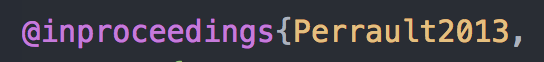
\includegraphics{figures/bibtexkey}

\subsection{How to get Bibtex References?}
The easiest way to find the Bibtex snippet you need for a given reference is to use Google Scholar~(\cite{Scholar}).
On the main page, type the name of the paper you are looking for.
\\

In the results page, locate the paper:
\begin{figure}[!h]
  \centering
    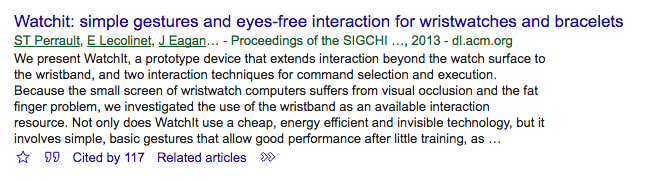
\includegraphics[width=0.9\textwidth]{figures/scholarrefexample.png}
  \caption{Example of result on Scholar}
  \label{fig:scholarref}
\end{figure}

On the last line of the result (shown in Figure~\ref{fig:scholarref}), there is a \textbf{''} symbol.
Clicking on it will display a pop-up.
\begin{figure}[!h]
  \centering
    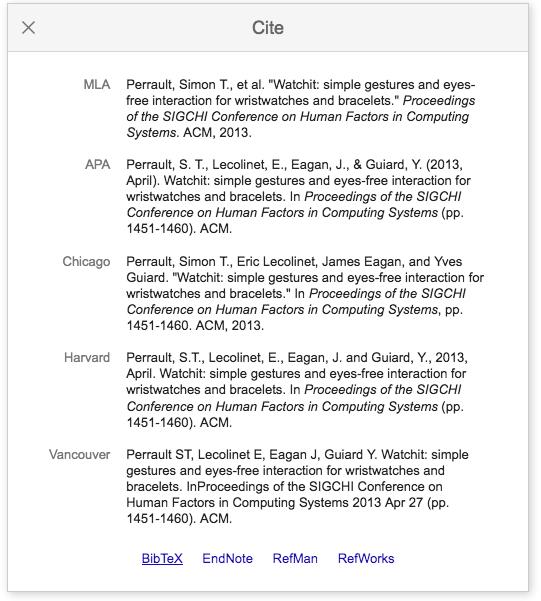
\includegraphics[width=0.7\textwidth]{figures/scholarpopup.png}
  \caption{Pop-up window with the possible citations}
  \label{fig:scholarpopup}
\end{figure}
\\

At the bottom (see Figure~\ref{fig:scholarpopup}), you will notice a ``Bibtex'' link. Click on it.
Scholar will then display a small block of text starting with @ symbol.
Copy and paste this snippet in your \texttt{biblio.bib} and you are done.
You may eventually want to check the citation key to something shorter.
\\

\textbf{You may get unexpected compilation errors with some references. The most common case is that the bibtex entry contains a DOI field, which in turn contains an underscore (\_).}
If that is the case, simply remove the DOI field (not a great practice but a good workaround).

\section{End of the Tips}
We are now done with the tips.
The next chapter contains more explanations and specificites of LaTeX{} and the template used here.
Good luck with your capstone report.

% \chapter{Chapter Title Here} % Main chapter title


\label{chapter2} % For referencing the chapter elsewhere, use \ref{Chapter1}

\epigraph{``Seriously, who puts stupid quotes at the beginning of a chapter? A quote alone will not give me more points on the report anyway.''}{\textit{You, dawn of the 3rd day}}

%----------------------------------------------------------------------------------------
We can reference other chapters, for example, here we refer to Chapter~\ref{chapter1}.

%----------------------------------------------------------------------------------------

% Define some commands to keep the formatting separated from the content
\newcommand{\keyword}[1]{\textbf{#1}}
\newcommand{\tabhead}[1]{\textbf{#1}}
\newcommand{\code}[1]{\texttt{#1}}
\newcommand{\file}[1]{\texttt{\bfseries#1}}
\newcommand{\option}[1]{\texttt{\itshape#1}}

%----------------------------------------------------------------------------------------

\section{Welcome and Thank You}
Welcome to this \LaTeX{} Thesis Template, a beautiful and easy to use template for writing a thesis using the \LaTeX{} typesetting system.

If you are writing a thesis (or will be in the future) and its subject is technical or mathematical (though it doesn't have to be), then creating it in \LaTeX{} is highly recommended as a way to make sure you can just get down to the essential writing without having to worry over formatting or wasting time arguing with your word processor.

\LaTeX{} is easily able to professionally typeset documents that run to hundreds or thousands of pages long. With simple mark-up commands, it automatically sets out the table of contents, margins, page headers and footers and keeps the formatting consistent and beautiful. One of its main strengths is the way it can easily typeset mathematics, even \emph{heavy} mathematics. Even if those equations are the most horribly twisted and most difficult mathematical problems that can only be solved on a super-computer, you can at least count on \LaTeX{} to make them look stunning.

%----------------------------------------------------------------------------------------

\section{Learning \LaTeX{}}

\LaTeX{} is not a \textsc{wysiwyg} (What You See is What You Get) program, unlike word processors such as Microsoft Word or Apple's Pages. Instead, a document written for \LaTeX{} is actually a simple, plain text file that contains \emph{no formatting}. You tell \LaTeX{} how you want the formatting in the finished document by writing in simple commands amongst the text, for example, if I want to use \emph{italic text for emphasis}, I write the \verb|\emph{text}| command and put the text I want in italics in between the curly braces. This means that \LaTeX{} is a \enquote{mark-up} language, very much like HTML.

\subsection{A (not so short) Introduction to \LaTeX{}}

If you are new to \LaTeX{}, there is a very good eBook -- freely available online as a PDF file -- called, \enquote{The Not So Short Introduction to \LaTeX{}}. The book's title is typically shortened to just \emph{lshort}. You can download the latest version (as it is occasionally updated) from here:
\url{http://www.ctan.org/tex-archive/info/lshort/english/lshort.pdf}

It is also available in several other languages. Find yours from the list on this page: \url{http://www.ctan.org/tex-archive/info/lshort/}

It is recommended to take a little time out to learn how to use \LaTeX{} by creating several, small `test' documents, or having a close look at several templates on:\\
\url{http://www.LaTeXTemplates.com}\\
Making the effort now means you're not stuck learning the system when what you \emph{really} need to be doing is writing your thesis.

\subsection{A Short Math Guide for \LaTeX{}}

If you are writing a technical or mathematical thesis, then you may want to read the document by the AMS (American Mathematical Society) called, \enquote{A Short Math Guide for \LaTeX{}}. It can be found online here:
\url{http://www.ams.org/tex/amslatex.html}
under the \enquote{Additional Documentation} section towards the bottom of the page.

\subsection{Common \LaTeX{} Math Symbols}
There are a multitude of mathematical symbols available for \LaTeX{} and it would take a great effort to learn the commands for them all. The most common ones you are likely to use are shown on this page:
\url{http://www.sunilpatel.co.uk/latex-type/latex-math-symbols/}

You can use this page as a reference or crib sheet, the symbols are rendered as large, high quality images so you can quickly find the \LaTeX{} command for the symbol you need.

\subsection{\LaTeX{} on a Mac}

The \LaTeX{} distribution is available for many systems including Windows, Linux and Mac OS X. The package for OS X is called MacTeX and it contains all the applications you need -- bundled together and pre-customized -- for a fully working \LaTeX{} environment and work flow.

MacTeX includes a custom dedicated \LaTeX{} editor called TeXShop for writing your `\file{.tex}' files and BibDesk: a program to manage your references and create your bibliography section just as easily as managing songs and creating playlists in iTunes.

%----------------------------------------------------------------------------------------

\section{Getting Started with this Template}

If you are familiar with \LaTeX{}, then you should explore the directory structure of the template and then proceed to place your own information into the \emph{THESIS INFORMATION} block of the \file{main.tex} file. You can then modify the rest of this file to your unique specifications based on your degree/university. Section \ref{FillingFile} on page \pageref{FillingFile} will help you do this. Make sure you also read section \ref{ThesisConventions} about thesis conventions to get the most out of this template.

If you are new to \LaTeX{} it is recommended that you carry on reading through the rest of the information in this document.

Before you begin using this template you should ensure that its style complies with the thesis style guidelines imposed by your institution. In most cases this template style and layout will be suitable. If it is not, it may only require a small change to bring the template in line with your institution's recommendations. These modifications will need to be done on the \file{MastersDoctoralThesis.cls} file.

\subsection{About this Template}

This \LaTeX{} Thesis Template is originally based and created around a \LaTeX{} style file created by Steve R.\ Gunn from the University of Southampton (UK), department of Electronics and Computer Science. You can find his original thesis style file at his site, here:
\url{http://www.ecs.soton.ac.uk/~srg/softwaretools/document/templates/}

Steve's \file{ecsthesis.cls} was then taken by Sunil Patel who modified it by creating a skeleton framework and folder structure to place the thesis files in. The resulting template can be found on Sunil's site here:
\url{http://www.sunilpatel.co.uk/thesis-template}

Sunil's template was made available through \url{http://www.LaTeXTemplates.com} where it was modified many times based on user requests and questions. Version 2.0 and onwards of this template represents a major modification to Sunil's template and is, in fact, hardly recognisable. The work to make version 2.0 possible was carried out by \href{mailto:vel@latextemplates.com}{Vel} and Johannes Böttcher.

%----------------------------------------------------------------------------------------

\section{What this Template Includes}

\subsection{Folders}

This template comes as a single zip file that expands out to several files and folders. The folder names are mostly self-explanatory:

\keyword{Appendices} -- this is the folder where you put the appendices. Each appendix should go into its own separate \file{.tex} file. An example and template are included in the directory.

\keyword{Chapters} -- this is the folder where you put the thesis chapters. A thesis usually has about six chapters, though there is no hard rule on this. Each chapter should go in its own separate \file{.tex} file and they can be split as:
\begin{itemize}
\item Chapter 1: Introduction to the thesis topic
\item Chapter 2: Background information and theory
\item Chapter 3: (Laboratory) experimental setup
\item Chapter 4: Details of experiment 1
\item Chapter 5: Details of experiment 2
\item Chapter 6: Discussion of the experimental results
\item Chapter 7: Conclusion and future directions
\end{itemize}
This chapter layout is specialised for the experimental sciences, your discipline may be different.

\keyword{Figures} -- this folder contains all figures for the thesis. These are the final images that will go into the thesis document.

\subsection{Files}

Included are also several files, most of them are plain text and you can see their contents in a text editor. After initial compilation, you will see that more auxiliary files are created by \LaTeX{} or BibTeX and which you don't need to delete or worry about:

\keyword{example.bib} -- this is an important file that contains all the bibliographic information and references that you will be citing in the thesis for use with BibTeX. You can write it manually, but there are reference manager programs available that will create and manage it for you. Bibliographies in \LaTeX{} are a large subject and you may need to read about BibTeX before starting with this. Many modern reference managers will allow you to export your references in BibTeX format which greatly eases the amount of work you have to do.

\keyword{MastersDoctoralThesis.cls} -- this is an important file. It is the class file that tells \LaTeX{} how to format the thesis.

\keyword{main.pdf} -- this is your beautifully typeset thesis (in the PDF file format) created by \LaTeX{}. It is supplied in the PDF with the template and after you compile the template you should get an identical version.

\keyword{main.tex} -- this is an important file. This is the file that you tell \LaTeX{} to compile to produce your thesis as a PDF file. It contains the framework and constructs that tell \LaTeX{} how to layout the thesis. It is heavily commented so you can read exactly what each line of code does and why it is there. After you put your own information into the \emph{THESIS INFORMATION} block -- you have now started your thesis!

Files that are \emph{not} included, but are created by \LaTeX{} as auxiliary files include:

\keyword{main.aux} -- this is an auxiliary file generated by \LaTeX{}, if it is deleted \LaTeX{} simply regenerates it when you run the main \file{.tex} file.

\keyword{main.bbl} -- this is an auxiliary file generated by BibTeX, if it is deleted, BibTeX simply regenerates it when you run the \file{main.aux} file. Whereas the \file{.bib} file contains all the references you have, this \file{.bbl} file contains the references you have actually cited in the thesis and is used to build the bibliography section of the thesis.

\keyword{main.blg} -- this is an auxiliary file generated by BibTeX, if it is deleted BibTeX simply regenerates it when you run the main \file{.aux} file.

\keyword{main.lof} -- this is an auxiliary file generated by \LaTeX{}, if it is deleted \LaTeX{} simply regenerates it when you run the main \file{.tex} file. It tells \LaTeX{} how to build the \emph{List of Figures} section.

\keyword{main.log} -- this is an auxiliary file generated by \LaTeX{}, if it is deleted \LaTeX{} simply regenerates it when you run the main \file{.tex} file. It contains messages from \LaTeX{}, if you receive errors and warnings from \LaTeX{}, they will be in this \file{.log} file.

\keyword{main.lot} -- this is an auxiliary file generated by \LaTeX{}, if it is deleted \LaTeX{} simply regenerates it when you run the main \file{.tex} file. It tells \LaTeX{} how to build the \emph{List of Tables} section.

\keyword{main.out} -- this is an auxiliary file generated by \LaTeX{}, if it is deleted \LaTeX{} simply regenerates it when you run the main \file{.tex} file.

So from this long list, only the files with the \file{.bib}, \file{.cls} and \file{.tex} extensions are the most important ones. The other auxiliary files can be ignored or deleted as \LaTeX{} and BibTeX will regenerate them.

%----------------------------------------------------------------------------------------

\section{Filling in Your Information in the \file{main.tex} File}\label{FillingFile}

You will need to personalise the thesis template and make it your own by filling in your own information. This is done by editing the \file{main.tex} file in a text editor or your favourite LaTeX environment.

Open the file and scroll down to the third large block titled \emph{THESIS INFORMATION} where you can see the entries for \emph{University Name}, \emph{Department Name}, etc \ldots

Fill out the information about yourself, your group and institution. You can also insert web links, if you do, make sure you use the full URL, including the \code{http://} for this. If you don't want these to be linked, simply remove the \verb|\href{url}{name}| and only leave the name.

When you have done this, save the file and recompile \code{main.tex}. All the information you filled in should now be in the PDF, complete with web links. You can now begin your thesis proper!

%----------------------------------------------------------------------------------------

\section{The \code{main.tex} File Explained}

The \file{main.tex} file contains the structure of the thesis. There are plenty of written comments that explain what pages, sections and formatting the \LaTeX{} code is creating. Each major document element is divided into commented blocks with titles in all capitals to make it obvious what the following bit of code is doing. Initially there seems to be a lot of \LaTeX{} code, but this is all formatting, and it has all been taken care of so you don't have to do it.

Begin by checking that your information on the title page is correct. For the thesis declaration, your institution may insist on something different than the text given. If this is the case, just replace what you see with what is required in the \emph{DECLARATION PAGE} block.

Then comes a page which contains a funny quote. You can put your own, or quote your favourite scientist, author, person, and so on. Make sure to put the name of the person who you took the quote from.

Following this is the abstract page which summarises your work in a condensed way and can almost be used as a standalone document to describe what you have done. The text you write will cause the heading to move up so don't worry about running out of space.

Next come the acknowledgements. On this page, write about all the people who you wish to thank (not forgetting parents, partners and your advisor/supervisor).

The contents pages, list of figures and tables are all taken care of for you and do not need to be manually created or edited. The next set of pages are more likely to be optional and can be deleted since they are for a more technical thesis: insert a list of abbreviations you have used in the thesis, then a list of the physical constants and numbers you refer to and finally, a list of mathematical symbols used in any formulae. Making the effort to fill these tables means the reader has a one-stop place to refer to instead of searching the internet and references to try and find out what you meant by certain abbreviations or symbols.

The list of symbols is split into the Roman and Greek alphabets. Whereas the abbreviations and symbols ought to be listed in alphabetical order (and this is \emph{not} done automatically for you) the list of physical constants should be grouped into similar themes.

The next page contains a one line dedication. Who will you dedicate your thesis to?

Finally, there is the block where the chapters are included. Uncomment the lines (delete the \code{\%} character) as you write the chapters. Each chapter should be written in its own file and put into the \emph{Chapters} folder and named \file{Chapter1}, \file{Chapter2}, etc\ldots Similarly for the appendices, uncomment the lines as you need them. Each appendix should go into its own file and placed in the \emph{Appendices} folder.

After the preamble, chapters and appendices finally comes the bibliography. The bibliography style (called \option{authoryear}) is used for the bibliography and is a fully featured style that will even include links to where the referenced paper can be found online. Do not underestimate how grateful your reader will be to find that a reference to a paper is just a click away. Of course, this relies on you putting the URL information into the BibTeX file in the first place.

%----------------------------------------------------------------------------------------

\section{Thesis Features and Conventions}\label{ThesisConventions}

To get the best out of this template, there are a few conventions that you may want to follow.

One of the most important (and most difficult) things to keep track of in such a long document as a thesis is consistency. Using certain conventions and ways of doing things (such as using a Todo list) makes the job easier. Of course, all of these are optional and you can adopt your own method.

\subsection{Printing Format}

This thesis template is designed for double sided printing (i.e. content on the front and back of pages) as most theses are printed and bound this way. Switching to one sided printing is as simple as uncommenting the \option{oneside} option of the \code{documentclass} command at the top of the \file{main.tex} file. You may then wish to adjust the margins to suit specifications from your institution.

The headers for the pages contain the page number on the outer side (so it is easy to flick through to the page you want) and the chapter name on the inner side.

The text is set to 11 point by default with single line spacing, again, you can tune the text size and spacing should you want or need to using the options at the very start of \file{main.tex}. The spacing can be changed similarly by replacing the \option{singlespacing} with \option{onehalfspacing} or \option{doublespacing}.

\subsection{Using US Letter Paper}

The paper size used in the template is A4, which is the standard size in Europe. If you are using this thesis template elsewhere and particularly in the United States, then you may have to change the A4 paper size to the US Letter size. This can be done in the margins settings section in \file{main.tex}.

Due to the differences in the paper size, the resulting margins may be different to what you like or require (as it is common for institutions to dictate certain margin sizes). If this is the case, then the margin sizes can be tweaked by modifying the values in the same block as where you set the paper size. Now your document should be set up for US Letter paper size with suitable margins.

\subsection{References}

The \code{biblatex} package is used to format the bibliography and inserts references such as this one \parencite{Reference1}. The options used in the \file{main.tex} file mean that the in-text citations of references are formatted with the author(s) listed with the date of the publication. Multiple references are separated by semicolons (e.g. \parencite{Reference2, Reference1}) and references with more than three authors only show the first author with \emph{et al.} indicating there are more authors (e.g. \parencite{Reference3}). This is done automatically for you. To see how you use references, have a look at the \file{Chapter1.tex} source file. Many reference managers allow you to simply drag the reference into the document as you type.

Scientific references should come \emph{before} the punctuation mark if there is one (such as a comma or period). The same goes for footnotes\footnote{Such as this footnote, here down at the bottom of the page.}. You can change this but the most important thing is to keep the convention consistent throughout the thesis. Footnotes themselves should be full, descriptive sentences (beginning with a capital letter and ending with a full stop). The APA6 states: \enquote{Footnote numbers should be superscripted, [...], following any punctuation mark except a dash.} The Chicago manual of style states: \enquote{A note number should be placed at the end of a sentence or clause. The number follows any punctuation mark except the dash, which it precedes. It follows a closing parenthesis.}

The bibliography is typeset with references listed in alphabetical order by the first author's last name. This is similar to the APA referencing style. To see how \LaTeX{} typesets the bibliography, have a look at the very end of this document (or just click on the reference number links in in-text citations).

\subsubsection{A Note on bibtex}

The bibtex backend used in the template by default does not correctly handle unicode character encoding (i.e. "international" characters). You may see a warning about this in the compilation log and, if your references contain unicode characters, they may not show up correctly or at all. The solution to this is to use the biber backend instead of the outdated bibtex backend. This is done by finding this in \file{main.tex}: \option{backend=bibtex} and changing it to \option{backend=biber}. You will then need to delete all auxiliary BibTeX files and navigate to the template directory in your terminal (command prompt). Once there, simply type \code{biber main} and biber will compile your bibliography. You can then compile \file{main.tex} as normal and your bibliography will be updated. An alternative is to set up your LaTeX editor to compile with biber instead of bibtex, see \href{http://tex.stackexchange.com/questions/154751/biblatex-with-biber-configuring-my-editor-to-avoid-undefined-citations/}{here} for how to do this for various editors.

\subsection{Tables}

Tables are an important way of displaying your results, below is an example table which was generated with this code:

{\small
\begin{verbatim}
\begin{table}
\caption{The effects of treatments X and Y on the four groups studied.}
\label{tab:treatments}
\centering
\begin{tabular}{l l l}
\toprule
\tabhead{Groups} & \tabhead{Treatment X} & \tabhead{Treatment Y} \\
\midrule
1 & 0.2 & 0.8\\
2 & 0.17 & 0.7\\
3 & 0.24 & 0.75\\
4 & 0.68 & 0.3\\
\bottomrule\\
\end{tabular}
\end{table}
\end{verbatim}
}

\begin{table}
\caption{The effects of treatments X and Y on the four groups studied.}
\label{tab:treatments}
\centering
\begin{tabular}{l l l}
\toprule
\tabhead{Groups} & \tabhead{Treatment X} & \tabhead{Treatment Y} \\
\midrule
1 & 0.2 & 0.8\\
2 & 0.17 & 0.7\\
3 & 0.24 & 0.75\\
4 & 0.68 & 0.3\\
\bottomrule\\
\end{tabular}
\end{table}

You can reference tables with \verb|\ref{<label>}| where the label is defined within the table environment. See \file{Chapter1.tex} for an example of the label and citation (e.g. Table~\ref{tab:treatments}).

\subsection{Figures}

There will hopefully be many figures in your thesis (that should be placed in the \emph{Figures} folder). The way to insert figures into your thesis is to use a code template like this:
\begin{verbatim}
\begin{figure}
\centering
\includegraphics{Figures/Electron}
\decoRule
\caption[An Electron]{An electron (artist's impression).}
\label{fig:Electron}
\end{figure}
\end{verbatim}
Also look in the source file. Putting this code into the source file produces the picture of the electron that you can see in the figure below.

\begin{figure}[th]
\centering

\includegraphics{figures/electron}
\decoRule
\caption[An Electron]{An electron (artist's impression).}
\label{fig:Electron}
\end{figure}

Sometimes figures don't always appear where you write them in the source. The placement depends on how much space there is on the page for the figure. Sometimes there is not enough room to fit a figure directly where it should go (in relation to the text) and so \LaTeX{} puts it at the top of the next page. Positioning figures is the job of \LaTeX{} and so you should only worry about making them look good!

Figures usually should have captions just in case you need to refer to them (such as in Figure~\ref{fig:Electron}). The \verb|\caption| command contains two parts, the first part, inside the square brackets is the title that will appear in the \emph{List of Figures}, and so should be short. The second part in the curly brackets should contain the longer and more descriptive caption text.

The \verb|\decoRule| command is optional and simply puts an aesthetic horizontal line below the image. If you do this for one image, do it for all of them.

\LaTeX{} is capable of using images in pdf, jpg and png format.

\subsection{Typesetting mathematics}

If your thesis is going to contain heavy mathematical content, be sure that \LaTeX{} will make it look beautiful, even though it won't be able to solve the equations for you.

The \enquote{Not So Short Introduction to \LaTeX} (available on \href{http://www.ctan.org/tex-archive/info/lshort/english/lshort.pdf}{CTAN}) should tell you everything you need to know for most cases of typesetting mathematics. If you need more information, a much more thorough mathematical guide is available from the AMS called, \enquote{A Short Math Guide to \LaTeX} and can be downloaded from:
\url{ftp://ftp.ams.org/pub/tex/doc/amsmath/short-math-guide.pdf}

There are many different \LaTeX{} symbols to remember, luckily you can find the most common symbols in \href{http://ctan.org/pkg/comprehensive}{The Comprehensive \LaTeX~Symbol List}.

You can write an equation, which is automatically given an equation number by \LaTeX{} like this:
\begin{verbatim}
\begin{equation}
E = mc^{2}
\label{eqn:Einstein}
\end{equation}
\end{verbatim}

This will produce Einstein's famous energy-matter equivalence equation:
\begin{equation}
E = mc^{2}
\label{eqn:Einstein}
\end{equation}

All equations you write (which are not in the middle of paragraph text) are automatically given equation numbers by \LaTeX{}. If you don't want a particular equation numbered, use the unnumbered form:
\begin{verbatim}
\[ a^{2}=4 \]
\end{verbatim}

%----------------------------------------------------------------------------------------

\section{Sectioning and Subsectioning}

You should break your thesis up into nice, bite-sized sections and subsections. \LaTeX{} automatically builds a table of Contents by looking at all the \verb|\chapter{}|, \verb|\section{}|  and \verb|\subsection{}| commands you write in the source.

The Table of Contents should only list the sections to three (3) levels. A \verb|chapter{}| is level zero (0). A \verb|\section{}| is level one (1) and so a \verb|\subsection{}| is level two (2). In your thesis it is likely that you will even use a \verb|subsubsection{}|, which is level three (3). The depth to which the Table of Contents is formatted is set within \file{MastersDoctoralThesis.cls}. If you need this changed, you can do it in \file{main.tex}.

%----------------------------------------------------------------------------------------

\section{In Closing}

You have reached the end of this mini-guide. You can now rename or overwrite this pdf file and begin writing your own \file{Chapter1.tex} and the rest of your thesis. The easy work of setting up the structure and framework has been taken care of for you. It's now your job to fill it out!

Good luck and have lots of fun!

\begin{flushright}
Guide written by ---\\
Sunil Patel: \href{http://www.sunilpatel.co.uk}{www.sunilpatel.co.uk}\\
Vel: \href{http://www.LaTeXTemplates.com}{LaTeXTemplates.com}
\end{flushright}


%----------------------------------------------------------------------------------------
%	BIBLIOGRAPHY
%----------------------------------------------------------------------------------------

\printbibliography[heading=bibintoc]

%----------------------------------------------------------------------------------------
%	THESIS CONTENT - APPENDICES
%----------------------------------------------------------------------------------------

\appendix % Cue to tell LaTeX that the following "chapters" are Appendices

% Include the appendices of the thesis as separate files from the Appendices folder
% Uncomment the lines as you write the Appendices

 % Appendix A

\chapter{Frequently Asked Questions} % Main appendix title

\label{AppendixA} % For referencing this appendix elsewhere, use \ref{AppendixA}

\section{How do I change the colors of links?}

The color of links can be changed to your liking using:

{\small\verb!\hypersetup{urlcolor=red}!}, or

{\small\verb!\hypersetup{citecolor=green}!}, or

{\small\verb!\hypersetup{allcolor=blue}!}.

\noindent If you want to completely hide the links, you can use:

{\small\verb!\hypersetup{allcolors=.}!}, or even better: 

{\small\verb!\hypersetup{hidelinks}!}.

\noindent If you want to have obvious links in the PDF but not the printed text, use:

{\small\verb!\hypersetup{colorlinks=false}!}.
